\section{Scheduling}

Scheduling: Zuteilug der CPU (Betriebsmittel) an Threads/Prozesse

\subsection{Wann wird der Scheduler aktiv}
\begin{itemize}
    \item neuer Prozess entsteht
    \item aktiver Prozess endet
    \item Prozess wg. I/O blockiert
    \item Zeitquantum is aufgebraucht
    \item Interrupt tritt auf
\end{itemize}

\subsection{Scheduling-Prinzipien}
\begin{itemize}
    \item Kooperativ
    \item Präemptiv
    \item Batch
    \begin{itemize}
        \item FCFS
        \begin{itemize}
            \item nicht Präemptiv
            \item minimiert durchschnittliche Verweilzeit
            \item I/O ineffizient
        \end{itemize}
        \item SJF und SRT
        \begin{itemize}
            \item minimiert Wartezeit
            \item starvation
        \end{itemize}
        \item Prioritäten
    \end{itemize}
\end{itemize}

\subsection{Kriterien}

\subsubsection{Anwendersicht}
\begin{itemize}
    \item Ausführungsdauer (Prozess-Gesamtlaufzeit)
    \item Reaktionszeit (Reaktionen auf Benutzerinteraktionen)
    \item Deadlines
    \item Vorhersagbarkeit (gleichartige Prozesse)
    \item Proportionalität
\end{itemize}

\subsubsection{Systemsicht}
\begin{itemize}
    \item Durchsatz (Prozesse pro Zeit)
    \item Prozessauslastung (Cycles pro Zeit)
    \item Fairness (keine starvation)
    \item Prioritäten
    \item Resourcen Fairness
\end{itemize}

\subsubsection{Wahl des Quantums}
\begin{itemize}
    \item zu groß: Latency
    \item zu klein: Overhead durch Kontextwechsel
    \item typisch: 10-100ms
\end{itemize}

\subsection{Round Robin und I/O}
\subsubsection{Virtual Round Robin}
\begin{figure}[ht!]
    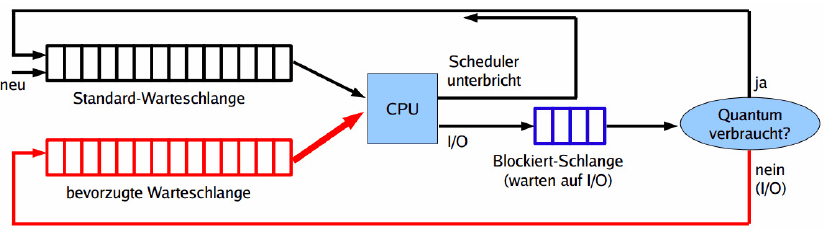
\includegraphics[scale=.4]{pics/virtual_round_robin}
    \caption{Virtual round robin prinzip}
\end{figure}

\subsubsection{Prioritätsbasiert}
\begin{itemize}
    \item Dynamisch (+ variable Quantenlänge): z.B. Aging (~SJF)
    \item Multilevel Scheduling
\end{itemize}

\textbf{Priority-Inversion:}
\begin{figure}[ht!]
    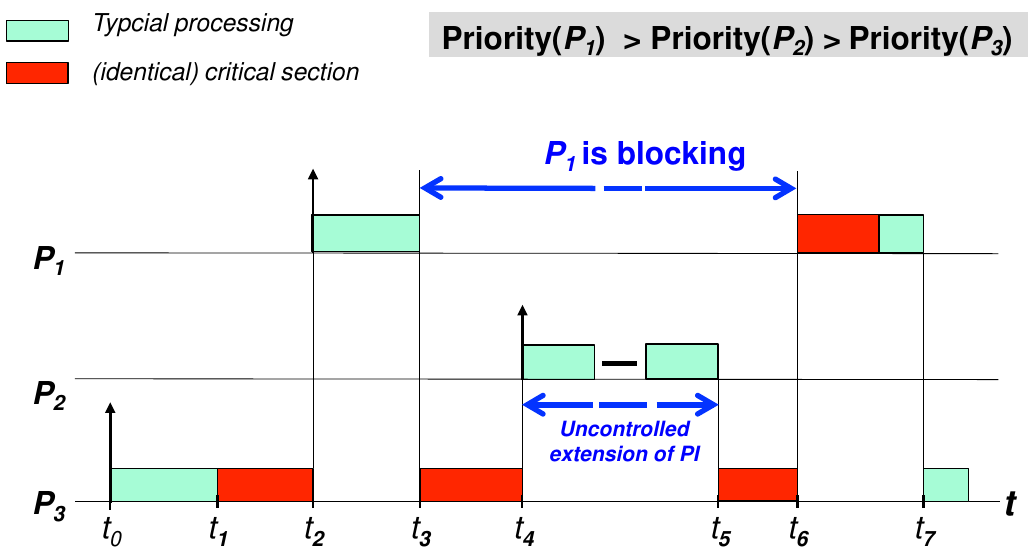
\includegraphics[scale=.3]{pics/priority_inversion}
    \caption{Beispiel für Priority-Inversion}
\end{figure}

\subsection{Formeln}
\subsubsection{Burstdauer}
\begin{itemize}
    \item $S_{n+1} = \frac{1}{n} \sum_{i=1}^n T_i = \frac{1}{n} T_n + \frac{n-1}{n} S_n$
    \item $S_{n+1} = \alpha T_n + (1-\alpha) S_n; \alpha \in [0,1]$
\end{itemize}

\subsection{Linux Prioritäten: nice}
\begin{itemize}
    \item nice, renice
    \item NeuePrio = Basis-Prio + CPU-Nutzung/2 + nice-value
\end{itemize}